\documentclass[11pt,a4paper]{report}
\usepackage[textwidth=37em,vmargin=30mm]{geometry}
\usepackage{calc,xunicode,amsmath,amssymb,paralist,enumitem,tabu,booktabs,datetime2,xeCJK,xeCJKfntef,listings}
\usepackage{tocloft,fancyhdr,tcolorbox,xcolor,graphicx,eso-pic,xltxtra,xelatexemoji}

\newcommand{\envyear}[0]{2025}
\newcommand{\envdatestr}[0]{2025-10-01}
\newcommand{\envfinaldir}[0]{webdb/2025/20251001/final}

\usepackage[hidelinks]{hyperref}
\hypersetup{
    colorlinks=false,
    pdfpagemode=FullScreen,
    pdftitle={Web Digest - \envdatestr}
}

\setlength{\cftbeforechapskip}{10pt}
\renewcommand{\cftchapfont}{\rmfamily\bfseries\large\raggedright}
\setlength{\cftbeforesecskip}{2pt}
\renewcommand{\cftsecfont}{\sffamily\small\raggedright}

\setdefaultleftmargin{2em}{2em}{1em}{1em}{1em}{1em}

\usepackage{xeCJK,xeCJKfntef}
\xeCJKsetup{PunctStyle=plain,RubberPunctSkip=false,CJKglue=\strut\hskip 0pt plus 0.1em minus 0.05em,CJKecglue=\strut\hskip 0.22em plus 0.2em}
\XeTeXlinebreaklocale "zh"
\XeTeXlinebreakskip = 0pt


\setmainfont{Brygada 1918}
\setromanfont{Brygada 1918}
\setsansfont{IBM Plex Sans}
\setmonofont{JetBrains Mono NL}
\setCJKmainfont{Noto Serif CJK SC}
\setCJKromanfont{Noto Serif CJK SC}
\setCJKsansfont{Noto Sans CJK SC}
\setCJKmonofont{Noto Sans CJK SC}

\setlength{\parindent}{0pt}
\setlength{\parskip}{8pt}
\linespread{1.15}

\lstset{
	basicstyle=\ttfamily\footnotesize,
	numbersep=5pt,
	backgroundcolor=\color{black!5},
	showspaces=false,
	showstringspaces=false,
	showtabs=false,
	tabsize=2,
	captionpos=b,
	breaklines=true,
	breakatwhitespace=true,
	breakautoindent=true,
	linewidth=\textwidth
}






\newcommand{\coverpic}[2]{
    % argv: itemurl, authorname
    Cover photo by #2~~(\href{#1}{#1})
}
\newcommand{\makeheader}[0]{
    \begin{titlepage}
        % \newgeometry{hmargin=15mm,tmargin=21mm,bmargin=12mm}
        \begin{center}
            
            \rmfamily\scshape
            \fontspec{BaskervilleF}
            \fontspec{Old Standard}
            \fontsize{59pt}{70pt}\selectfont
            WEB\hfill DIGEST
            
            \vfill
            % \vskip 30pt
            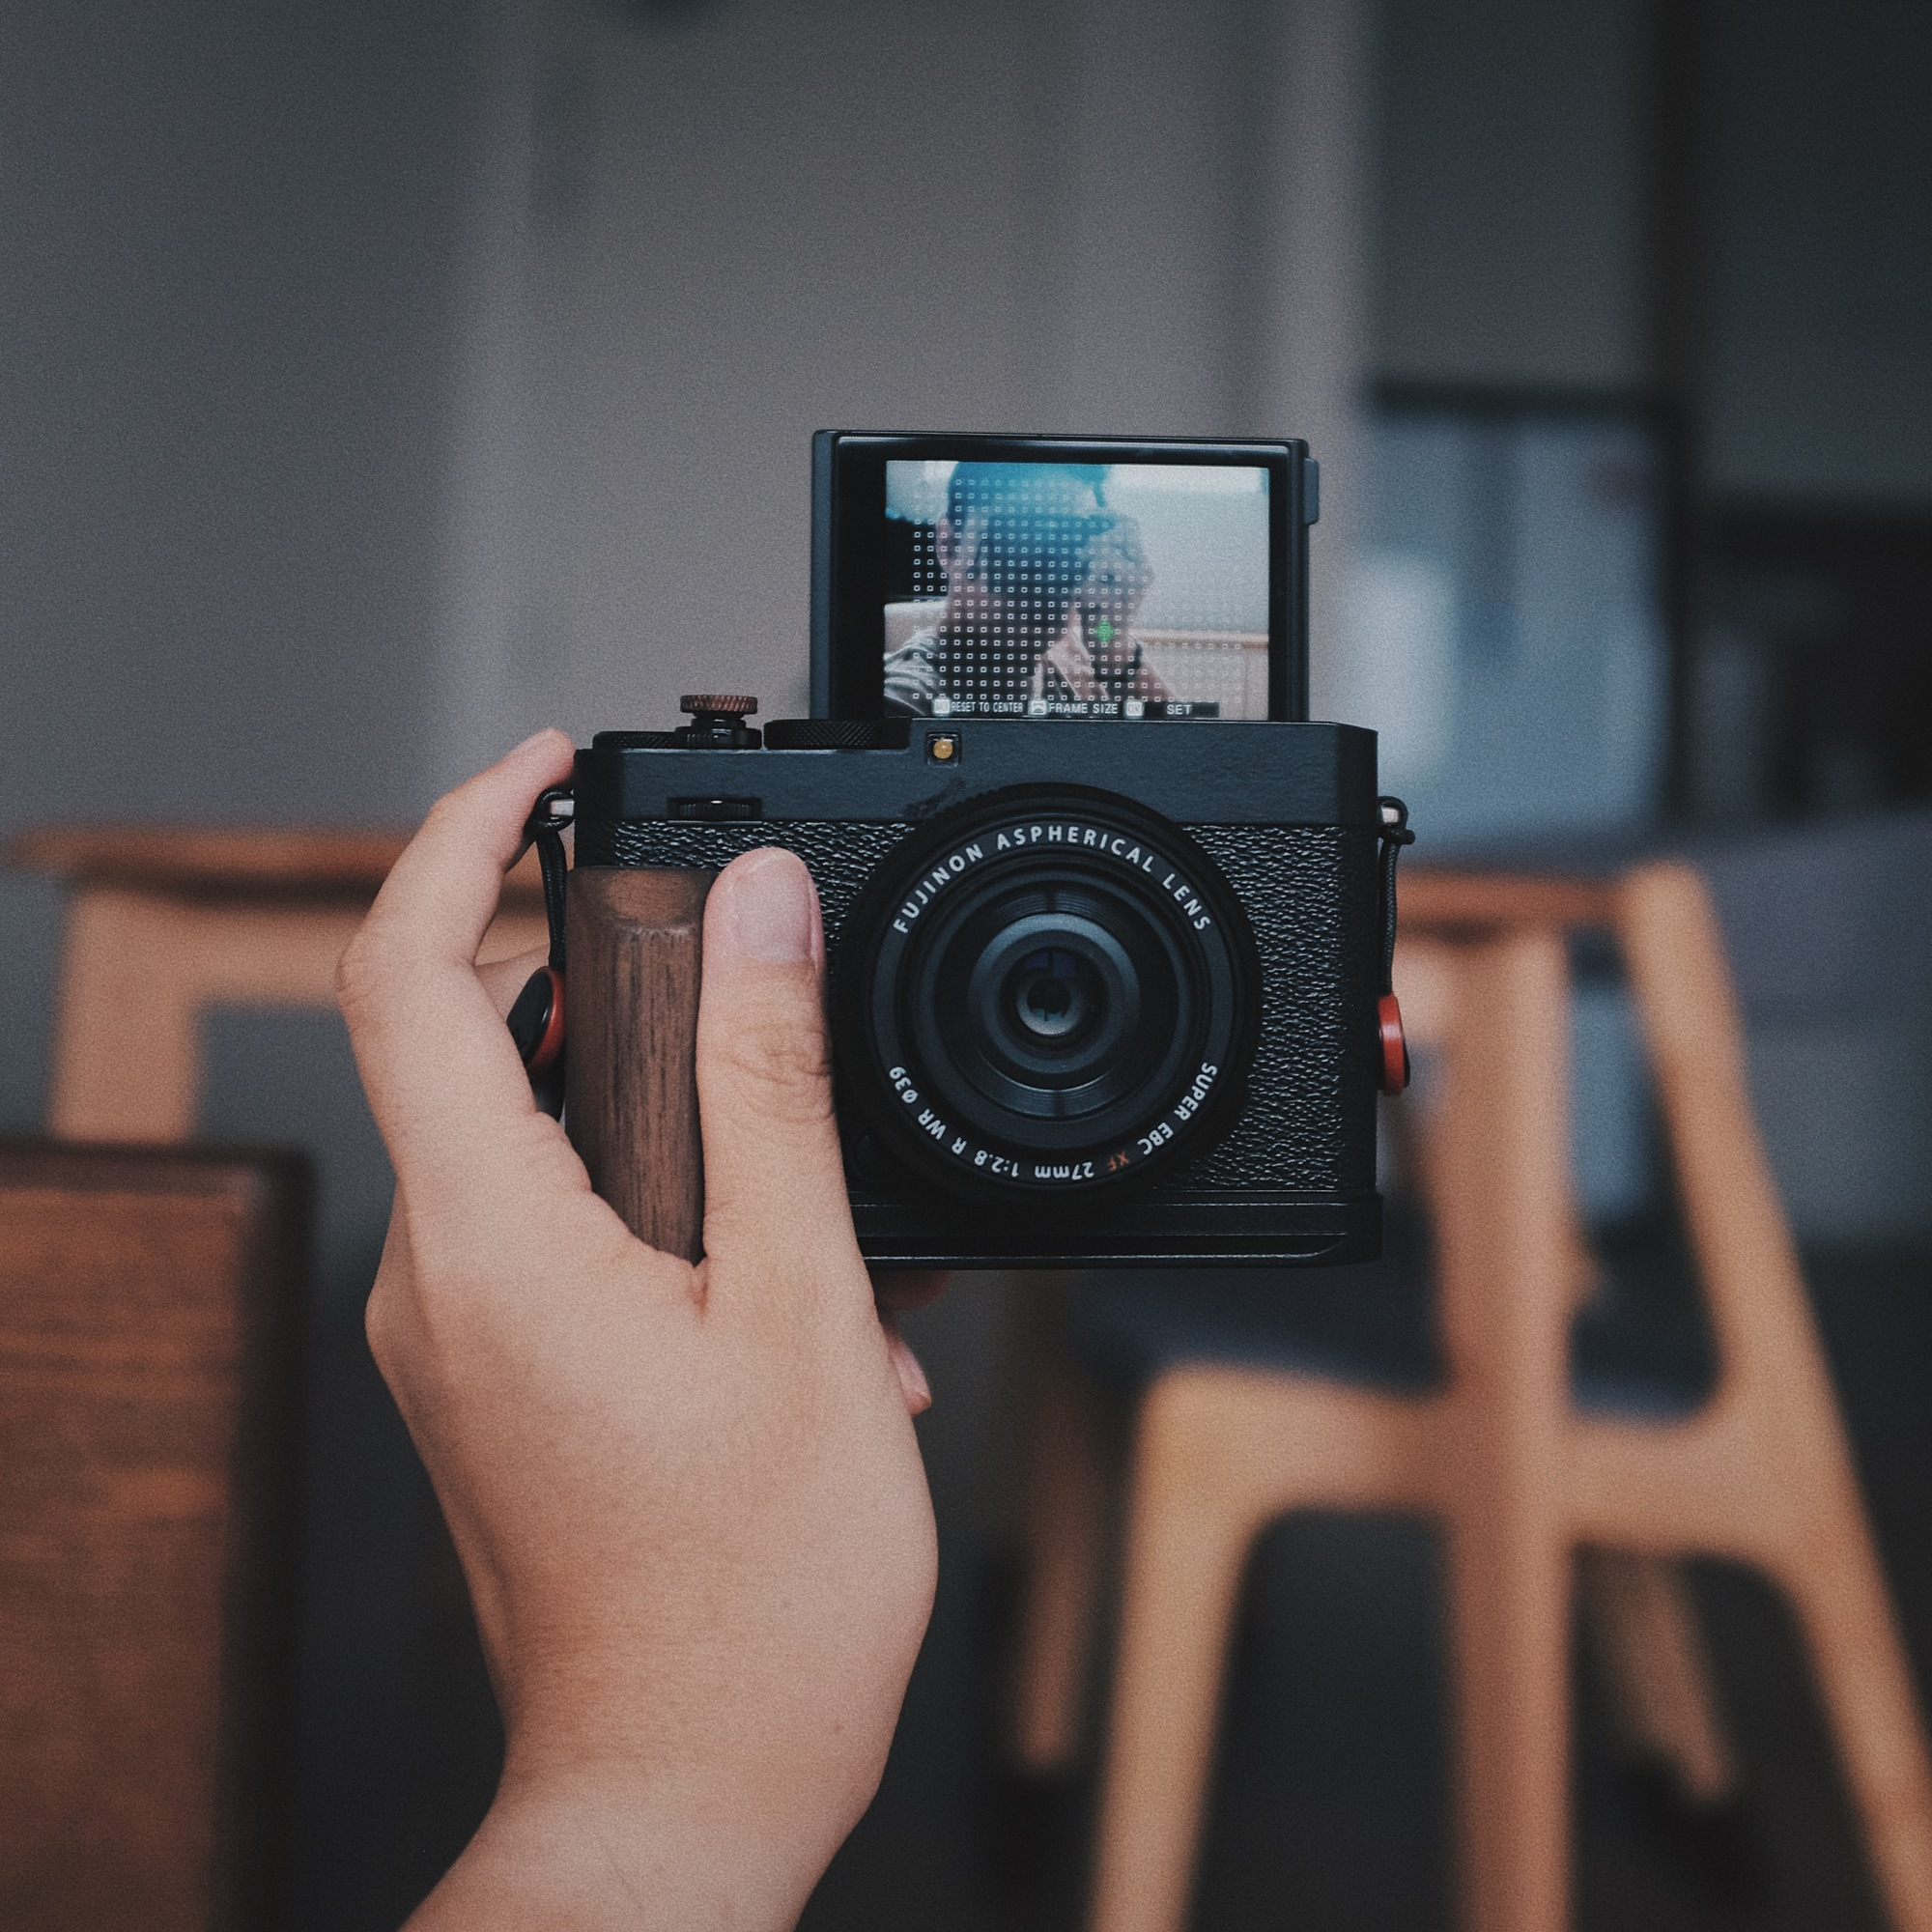
\includegraphics[width=\linewidth]{\envfinaldir/coverpic-prod.jpg}\par
            % \vskip 30pt
            \vfill

            \normalsize\rmfamily\scshape
            \copyright{} The Web Digest Project \hfill\large \envdatestr
        \end{center}
    \end{titlepage}
    % \restoregeometry
}
\newcommand{\simplehref}[1]{%
    \textcolor{blue!80!green}{\href{#1}{#1}}%
}
\renewcommand{\contentsname}{\center\Huge\sffamily\bfseries Contents\par\vskip 20pt}
\newcounter{ipartcounter}
\setcounter{ipartcounter}{0}
\newcommand{\ipart}[1]{
    % \vskip 20pt
    \clearpage
    \stepcounter{ipartcounter}
    \phantomsection
    \addcontentsline{toc}{chapter}{#1}
    % \begin{center}
    %     \Huge
    %     \sffamily\bfseries
    %     #1
    % \end{center}
    % \vskip 20pt plus 7pt
}
\newcounter{ichaptercounter}
\setcounter{ichaptercounter}{0}
\newcommand{\ichapter}[1]{
    % \vskip 20pt
    \clearpage
    \stepcounter{ichaptercounter}
    \phantomsection
    \addcontentsline{toc}{section}{\numberline{\arabic{ichaptercounter}}#1}
    \begin{center}
        \Huge
        \sffamily\bfseries
        #1
    \end{center}
    \vskip 20pt plus 7pt
}
\newcommand{\entrytitlefont}[1]{\subsection*{\raggedright\Large\sffamily\bfseries#1}}
\newcommand{\entryitemGeneric}[2]{
    % argv: title, url
    \parbox{\linewidth}{
        \entrytitlefont{#1}\par\vskip 5pt
        \footnotesize\ttfamily\mdseries
        \simplehref{#2}
    }\vskip 11pt plus 11pt minus 1pt
}
\newcommand{\entryitemGithub}[3]{
    % argv: title, url, desc
    \parbox{\linewidth}{
        \entrytitlefont{#1}\par\vskip 5pt
        \footnotesize\ttfamily\mdseries
        \simplehref{#2}\par\vskip 5pt
        \small\rmfamily\mdseries#3
    }\vskip 11pt plus 11pt minus 1pt
}
\newcommand{\entryitemAp}[3]{
    % argv: title, url, desc
    \parbox{\linewidth}{
        \entrytitlefont{#1}\par\vskip 5pt
        \footnotesize\ttfamily\mdseries
        \simplehref{#2}\par\vskip 5pt
        \small\rmfamily\mdseries#3
    }\vskip 11pt plus 11pt minus 1pt
}
\newcommand{\entryitemHackernews}[3]{
    % argv: title, hnurl, rawurl
    % \parbox{\linewidth}{
    %     \entrytitlefont{#1}\par\vskip 5pt
    %     \footnotesize\ttfamily\mdseries
    %     \simplehref{#3}\par
    %     \textcolor{black!50}{\href{#2}{#2}}
    % }\vskip 11pt plus 11pt minus 1pt
    \begin{minipage}{\linewidth}
            \entrytitlefont{#1}\par\vskip 5pt
            \footnotesize\ttfamily\mdseries
            \simplehref{#3}\par
            \textcolor{black!50}{\href{#2}{#2}}
    \end{minipage}\par\vskip 11pt plus 11pt minus 1pt
}







\begin{document}

\makeheader

\tableofcontents\clearpage




\ipart{Developers}
\ichapter{Hacker News}
\entryitemTwoLinks{Atuin Desktop: Runbooks That Run – Now Open Source}{https://news.ycombinator.com/item?id=45431001}{https://blog.atuin.sh/atuin-desktop-open-source/}

\entryitemTwoLinks{Inflammation now predicts heart disease more strongly than cholesterol}{https://news.ycombinator.com/item?id=45430498}{https://www.empirical.health/blog/inflammation-and-heart-health/}

\entryitemTwoLinks{Boeing has started working on a 737 MAX replacement}{https://news.ycombinator.com/item?id=45428482}{https://www.wsj.com/business/airlines/boeing-has-started-working-on-a-737-max-replacement-40a110df}

\entryitemTwoLinks{Sora 2}{https://news.ycombinator.com/item?id=45428122}{https://openai.com/index/sora-2/}

\entryitemTwoLinks{Sora 2}{https://news.ycombinator.com/item?id=45427982}{https://openai.com/index/sora-2/}

\entryitemTwoLinks{Show HN: Sculptor, the Missing UI for Claude Code}{https://news.ycombinator.com/item?id=45427697}{https://imbue.com/sculptor/}

\entryitemTwoLinks{Extract-0: A specialized language model for document information extraction}{https://news.ycombinator.com/item?id=45427634}{https://arxiv.org/abs/2509.22906}

\entryitemTwoLinks{Launch HN: Airweave (YC X25) – Let agents search any app}{https://news.ycombinator.com/item?id=45427482}{https://github.com/airweave-ai/airweave}

\entryitemTwoLinks{Leaked Apple M5 9 core Geekbench scores}{https://news.ycombinator.com/item?id=45427197}{https://browser.geekbench.com/v6/cpu/14173685}

\entryitemTwoLinks{Cerebras systems raises \$1.1B Series G}{https://news.ycombinator.com/item?id=45427111}{https://www.cerebras.ai/press-release/series-g}

\entryitemTwoLinks{Correctness and composability bugs in the Julia ecosystem (2022)}{https://news.ycombinator.com/item?id=45427021}{https://yuri.is/not-julia/}

\entryitemTwoLinks{Designing agentic loops}{https://news.ycombinator.com/item?id=45426680}{https://simonwillison.net/2025/Sep/30/designing-agentic-loops/}

\entryitemTwoLinks{Kagi News}{https://news.ycombinator.com/item?id=45426490}{https://blog.kagi.com/kagi-news}

\entryitemTwoLinks{How the AI bubble ate Y Combinator}{https://news.ycombinator.com/item?id=45426205}{https://www.inc.com/sam-blum/how-the-ai-bubble-ate-y-combinator/91240632}

\entryitemTwoLinks{Selling Lemons}{https://news.ycombinator.com/item?id=45425746}{https://frankchimero.com/blog/2025/selling-lemons/}

\entryitemTwoLinks{dgsh – Directed Graph Shell}{https://news.ycombinator.com/item?id=45425298}{https://www2.dmst.aueb.gr/dds/sw/dgsh/}

\entryitemTwoLinks{An opinionated critique of Duolingo}{https://news.ycombinator.com/item?id=45425061}{https://isomorphism.xyz/blog/2025/duolingo/}

\entryitemTwoLinks{Imgur pulls out of UK as data watchdog threatens fine}{https://news.ycombinator.com/item?id=45424888}{https://www.express.co.uk/news/uk/2115228/image-site-imgur-pulls-out}

\entryitemTwoLinks{Founder sentenced to seven years in prison for fraudulent sale to JPMorgan}{https://news.ycombinator.com/item?id=45424827}{https://www.cnn.com/2025/09/30/business/charlie-javice-frank-sentenced-jpmorgan-intl}

\entryitemTwoLinks{Pasta Cooking Time}{https://news.ycombinator.com/item?id=45424704}{https://www.jefftk.com/p/pasta-cooking-time}\ichapter{Phoronix}
\entryitemGeneric{\hskip 0pt{}AMD Publishes Open-Source openSIL Code For Phoenix SoCs}{https://www.phoronix.com/news/AMD-openSIL-Phoenix}

\entryitemGeneric{\hskip 0pt{}Qualcomm Posts Initial Open-Source GPU Driver Patches For Adreno 800 Series}{https://www.phoronix.com/news/Linux-Kernel-Adreno-800-Patches}

\entryitemGeneric{\hskip 0pt{}Apple HFS/HFS+ File-System Drivers See More Fixes With Linux 6.18}{https://www.phoronix.com/news/Apple-HFS-Linux-6.18}

\entryitemGeneric{\hskip 0pt{}NVIDIA 580.95.05 Linux Driver Released}{https://www.phoronix.com/news/NVIDIA-580.95.05-Linux-Driver}

\entryitemGeneric{\hskip 0pt{}Linux's New "Transitional" Feature A Long Overdue Improvement For Kernel Configurations}{https://www.phoronix.com/news/Linux-6.18-Transitional}

\entryitemGeneric{\hskip 0pt{}XFS Removes Some Old Mount Options \& Enables Fsck By Default For Linux 6.18}{https://www.phoronix.com/news/Linux-6.18-XFS}

\entryitemGeneric{\hskip 0pt{}Intel Linux Setbacks, Linux Kernel Drama \& Other Q3 Highlights}{https://www.phoronix.com/news/Q3-2025-Linux-News}

\entryitemGeneric{\hskip 0pt{}Linux 6.18 Continues Refining IEEE-1394 Firewire Support In 2025}{https://www.phoronix.com/news/Linux-6.18-Firewire}

\entryitemGeneric{\hskip 0pt{}Today Is The Last Day On Our Autumn Deal To Help Support Linux Hardware Reviews}{https://www.phoronix.com/news/Autumn-2025-Deal-Ending-Soon}


\ipart{Developers~~~~(zh-Hans)}
\ichapter{Solidot}
\entryitemGeneric{\hskip 0pt{}阿富汗断网超过一天}{https://www.solidot.org/story?sid=82461}

\entryitemGeneric{\hskip 0pt{}Linus Torvalds 从 Linux 6.18 中完全移除了 Bcachefs }{https://www.solidot.org/story?sid=82460}

\entryitemGeneric{\hskip 0pt{}世界最高大桥花江峡谷大桥通车}{https://www.solidot.org/story?sid=82459}

\entryitemGeneric{\hskip 0pt{}CS 教授警告毕业生难找到工作}{https://www.solidot.org/story?sid=82458}

\entryitemGeneric{\hskip 0pt{}因 AI 需求大涨 DRAM 价格翻倍}{https://www.solidot.org/story?sid=82457}

\entryitemGeneric{\hskip 0pt{}微塑料可能削弱骨骼}{https://www.solidot.org/story?sid=82456}

\entryitemGeneric{\hskip 0pt{}阿富汗断网}{https://www.solidot.org/story?sid=82454}

\entryitemGeneric{\hskip 0pt{}投资财团以 550 亿美元私有化 EA}{https://www.solidot.org/story?sid=82453}

\entryitemGeneric{\hskip 0pt{}高糖芒果有助于降低糖尿病风险}{https://www.solidot.org/story?sid=82452}

\entryitemGeneric{\hskip 0pt{}日本公司研发出基于植物的生鱼片}{https://www.solidot.org/story?sid=82451}

\entryitemGeneric{\hskip 0pt{}RubyGems 社区发生项目控制权争夺战}{https://www.solidot.org/story?sid=82450}

\entryitemGeneric{\hskip 0pt{}加州公共和共享充电桩数量比加油站多 68\%}{https://www.solidot.org/story?sid=82449}

\entryitemGeneric{\hskip 0pt{}流浪行星发现有极光}{https://www.solidot.org/story?sid=82448}

\entryitemGeneric{\hskip 0pt{}瑞士周日公投以微弱多数批准电子身份证}{https://www.solidot.org/story?sid=82447}

\entryitemGeneric{\hskip 0pt{}F-Droid 发表声明反对 Google 验证应用开发者身份的要求}{https://www.solidot.org/story?sid=82446}

\entryitemGeneric{\hskip 0pt{}Linux 6.17 释出}{https://www.solidot.org/story?sid=82444}

\entryitemGeneric{\hskip 0pt{}百万年前的龙人化石或改写人类家谱}{https://www.solidot.org/story?sid=82443}

\entryitemGeneric{\hskip 0pt{}美国考虑要求芯片公司的芯片国内制造和进口各占一半}{https://www.solidot.org/story?sid=82442}

\entryitemGeneric{\hskip 0pt{}研究发现过去 15 年睡眠问题日益严重}{https://www.solidot.org/story?sid=82441}

\entryitemGeneric{\hskip 0pt{}电动汽车公司破产后,车主创建了非盈利组织确保汽车正常运行}{https://www.solidot.org/story?sid=82440}\ichapter{V2EX}
\entryitemGeneric{\hskip 0pt{}[问与答] 国庆还有哪些兄弟能坚持签到?}{https://www.v2ex.com/t/1162996}

\entryitemGeneric{\hskip 0pt{}[问与答] 求助,怎么恢复 Gitlab 账户}{https://www.v2ex.com/t/1162995}

\entryitemGeneric{\hskip 0pt{}[问与答] 银河录像局 Claude code 专业版赠送的 CODEX 额度}{https://www.v2ex.com/t/1162992}

\entryitemGeneric{\hskip 0pt{}[程序员] 感觉不少前端框架 版本升级似乎很不喜欢搞兼容?}{https://www.v2ex.com/t/1162990}

\entryitemGeneric{\hskip 0pt{}[iPad] 去年泄露 M4 MacBook Pro 的今天发了 M5 iPad Pro 的开箱视频}{https://www.v2ex.com/t/1162989}

\entryitemGeneric{\hskip 0pt{}[iPad] M5 iPad Pro 来了}{https://www.v2ex.com/t/1162988}

\entryitemGeneric{\hskip 0pt{}[Apple] Apple 导入图书过多以后就很难用}{https://www.v2ex.com/t/1162987}

\entryitemGeneric{\hskip 0pt{}[程序员] 迷茫的互联网码农,该不该走赴日这条路}{https://www.v2ex.com/t/1162986}

\entryitemGeneric{\hskip 0pt{}[Google] 网页版 Gmail 的代收功能将在 2026 年 1 月停止服务}{https://www.v2ex.com/t/1162985}

\entryitemGeneric{\hskip 0pt{}[问与答] 看片被老婆发现了,咋办?}{https://www.v2ex.com/t/1162981}

\entryitemGeneric{\hskip 0pt{}[程序员] JetBrains All Products Pack 累计十年续费达成~}{https://www.v2ex.com/t/1162980}

\entryitemGeneric{\hskip 0pt{}[Apple] 苹果开发者证书开个车,稳定第三年}{https://www.v2ex.com/t/1162979}

\entryitemGeneric{\hskip 0pt{}[买买买] 双十一快到了,电商平台又开始提前涨价了🤣}{https://www.v2ex.com/t/1162978}

\entryitemGeneric{\hskip 0pt{}[随想] 老家人为了面子太铺张了}{https://www.v2ex.com/t/1162977}

\entryitemGeneric{\hskip 0pt{}[问与答] 找了个兼职,前公司合作伙伴推荐的外派印度的工作,应该收多少钱?}{https://www.v2ex.com/t/1162976}

\entryitemGeneric{\hskip 0pt{}[问与答] 大佬们遇到各别被墙的站,需要开关下手机 Wi-Fi 就恢复,是什么问题呢?}{https://www.v2ex.com/t/1162974}

\entryitemGeneric{\hskip 0pt{}[程序员] 我记性很差,程序员是不是都这样?}{https://www.v2ex.com/t/1162973}

\entryitemGeneric{\hskip 0pt{}[分享创造] 一个简单好用的 PySide6 项目模板}{https://www.v2ex.com/t/1162972}

\entryitemGeneric{\hskip 0pt{}[计算机] 接上一篇 2025 年 10 月组装电脑}{https://www.v2ex.com/t/1162971}

\entryitemGeneric{\hskip 0pt{}[宽带症候群] Unifi 路由器下 IPv6 SLAAC 配置不定时断流问题}{https://www.v2ex.com/t/1162970}

\entryitemGeneric{\hskip 0pt{}[投资] 美股七大科技现在还值得买吗,推荐哪些 etf}{https://www.v2ex.com/t/1162969}

\entryitemGeneric{\hskip 0pt{}[分享创造] 做了一个 PSN 奖杯网站,前后端超过 99\%的代码均由 AI 编写}{https://www.v2ex.com/t/1162967}

\entryitemGeneric{\hskip 0pt{}[问与答] V 站可以加个设置屏蔽关键词的功能吗?好多帖真的连标题都不想看到}{https://www.v2ex.com/t/1162966}

\entryitemGeneric{\hskip 0pt{}[分享创造] 本地文生图提示词翻译与管理纯 html}{https://www.v2ex.com/t/1162965}

\entryitemGeneric{\hskip 0pt{}[Solana] VB 一直下跌,一直放着不操作,等一个奇迹}{https://www.v2ex.com/t/1162964}

\entryitemGeneric{\hskip 0pt{}[程序员] 什么情况, nvidia-cuda 源 下了干嘛?}{https://www.v2ex.com/t/1162963}

\entryitemGeneric{\hskip 0pt{}[问与答] 各位老哥们,帮我看下哪款办公 4K 显示器和好?有点犹豫...}{https://www.v2ex.com/t/1162962}

\entryitemGeneric{\hskip 0pt{}[Apple] M2 Mac mini 升到 macOS 26,有啥大坑不}{https://www.v2ex.com/t/1162961}

\entryitemGeneric{\hskip 0pt{}[问与答] 如果业余时间做一个类似 Eagle 这样的软件,该如何售卖?本身在职。。。}{https://www.v2ex.com/t/1162960}

\entryitemGeneric{\hskip 0pt{}[程序员] 程序员国庆假期时间安排}{https://www.v2ex.com/t/1162959}

\entryitemGeneric{\hskip 0pt{}[Flutter] 第一次写 flutter app 有个疑问}{https://www.v2ex.com/t/1162957}

\entryitemGeneric{\hskip 0pt{}[分享发现] 写了小脚本能 export/import zen-browser 中任意的一个 folder,这样我们就能用 git 管理我们每个任务所使用的网页了。}{https://www.v2ex.com/t/1162956}

\entryitemGeneric{\hskip 0pt{}[Android] 遇到一个问题 ,请大佬们帮看看,能解决或者提供解决思路的兄弟得来杯 Manner。}{https://www.v2ex.com/t/1162953}

\entryitemGeneric{\hskip 0pt{}[分享发现] 真的能被阿里系的 PC 端 Web 风控气死}{https://www.v2ex.com/t/1162952}

\entryitemGeneric{\hskip 0pt{}[问与答] 活泼和文静妹子选择困难后续,成学妹了!}{https://www.v2ex.com/t/1162951}

\entryitemGeneric{\hskip 0pt{}[问与答] 我有一个问题关于 Deepseek API 的问题,请大佬解惑}{https://www.v2ex.com/t/1162950}

\entryitemGeneric{\hskip 0pt{}[问与答] 十一有没有电子羊毛可以薅的?}{https://www.v2ex.com/t/1162949}

\entryitemGeneric{\hskip 0pt{}[V2EX] v 站网页是怎么调用到手机系统字体的}{https://www.v2ex.com/t/1162948}

\entryitemGeneric{\hskip 0pt{}[OpenAI] 有人知道 ZenMux 这个平台吗,看起来和 OpenRouter 差不多?}{https://www.v2ex.com/t/1162947}

\entryitemGeneric{\hskip 0pt{}[问与答] 感觉娃哈哈纯净水最近的味道不对啊}{https://www.v2ex.com/t/1162945}

\entryitemGeneric{\hskip 0pt{}[问与答] 有没有可以查询机票价格历史趋势的网站或应用?}{https://www.v2ex.com/t/1162944}

\entryitemGeneric{\hskip 0pt{}[问与答] gap 两年后,找到了两份工作,跪求大佬帮忙选一下哪个更合适}{https://www.v2ex.com/t/1162943}

\entryitemGeneric{\hskip 0pt{}[程序员] 抓取货拉拉预估费用}{https://www.v2ex.com/t/1162942}

\entryitemGeneric{\hskip 0pt{}[分享创造] 做了个免费\&无需注册 的 AI 头像生成产品}{https://www.v2ex.com/t/1162940}

\entryitemGeneric{\hskip 0pt{}[问与答] [户外装备] 我的户外三季徒步配置分享,欢迎户外大佬分享好物}{https://www.v2ex.com/t/1162939}

\entryitemGeneric{\hskip 0pt{}[Apple] 各位使用 ios26 的时候有没有遇到过自带输入法卡顿}{https://www.v2ex.com/t/1162938}

\entryitemGeneric{\hskip 0pt{}[问与答] 这个车位要不要买?}{https://www.v2ex.com/t/1162937}

\entryitemGeneric{\hskip 0pt{}[职场话题] 字节跳动连续三次在四面(HR)后挂,是什么意思?}{https://www.v2ex.com/t/1162936}

\entryitemGeneric{\hskip 0pt{}[问与答] trae、qoder、CodeBuddy 只有 trae 可以填 api?}{https://www.v2ex.com/t/1162935}

\entryitemGeneric{\hskip 0pt{}[Apple] 现在香港苹果专卖店有现货 iphone17pro 么}{https://www.v2ex.com/t/1162934}


\ipart{Generic News}







\clearpage
\leavevmode\vfill
\footnotesize

Copyright \copyright{} 2023-2025 Neruthes and other contributors.

This document is published with CC BY-NC-ND 4.0 license.

The entries listed in this newsletter may be copyrighted by their respective creators.

This newsletter is generated by the Web Digest project.

The newsletters are also delivered via Telegram channel \CJKunderline{\href{https://t.me/webdigestchannel}{https://t.me/webdigestchannel}}.\\
RSS feed is available at \CJKunderline{\href{https://webdigest.pages.dev/rss.xml}{https://webdigest.pages.dev/rss.xml}}.

This newsletter is available in PDF at
\CJKunderline{\href{https://webdigest.pages.dev/}{https://webdigest.pages.dev/}}.

The source code being used to generate this newsletter is available at\\
\CJKunderline{\href{https://github.com/neruthes/webdigest}{https://github.com/neruthes/webdigest}}.

This newsletter is also available in
\CJKunderline{\href{http://webdigest.pages.dev/readhtml/\envyear/WebDigest-20251001.html}{HTML}} and
\CJKunderline{\href{https://github.com/neruthes/webdigest/blob/master/markdown/\envyear/WebDigest-20251001.md}{Markdown}}.


\coverpic{https://unsplash.com/photos/interior-view-of-a-boat-with-seats-and-window-8x3B9WnQUgw}{Alexander Lunyov}


\end{document}
